
%%% Local Variables:
%%% mode: latex
%%% TeX-master: t
%%% End:

\chapter{硬件资源共享管理方法}
\label{chap:hwresman}

% 现有体系结构共享性能很差
由于缺少有效的硬件资源共享管理机制,现有服务器体系结构不能很好的在共享场景中工作。
不同应用无管理的访问共享硬件资源,产生资源竞争并造成严重的性能干扰,进而影响应用性能,
来自Intel的研究\cite{intel}表明在共享末级缓存上的资源竞争最多可造成30\%的性能干扰。
% 而现实需求又需要共享
随着计算机硬件技术不断发展,现在计算机所能提供的硬件资源不断增加,
单个应用很难充分利用全部硬件资源;
与此同时,云计算与移动互联网的发展与普及,应用的数量也在飞速增加。
通过虚拟化与容器等技术将不同应用运行在同一台服务器,提高服务器资源利用率,
应用共享硬件资源成为常态。
% 资源利用率与服务质量相冲突
%但应用服务质量与服务器资源率之间存在冲突,
在这种场景下为了保障延迟敏感型应用的性能不受影响,
这些延迟敏感型应用需要独占部分共享资源(如部署在单独的服务器\cite{}),
这造成数据中心服务器的资源利用率通常只有10\%-12\%。
如何为硬件资源提供灵活的共享管理方法,是解决服务器多应用共享的关键问题。


% 问题一:资源竞争点不断变化,需要统一的管理接口,control plane + ?PRM?
现有一些研究工作在单一硬件资源上提出共享管理的方法,
如在共享末级缓存上提出容量划分的方法\cite{},
在内存控制器上提供请求调度的方法\cite{},
Intel在其Xeon E5v3系列处理器中增加了末级缓存容量划分功能。
但是计算机内包含大量的共享硬件资源,不同应用混合后,会在不同的硬件上资源上产生竞争;
同时由于硬件资源之间存在关联,需要协调管理。
例如仅通过容量划分的方式解决在共享缓存中的资源竞争,
可能会造成在竞争点转移到内存控制器,这是由于
因此,为所有的硬件资源提供统一的共享管理接口,
并集中式的管理节点内的全部共享资源是必要的。

%
要实现硬件资源的共享管理,首先需要考虑如何监控资源用量,以及实时反馈。 % stab+ttab
现有体系结构实现中已实现的监控大都是针对片内资源,如处理器核IPC、分支预测正确率、XXX等,
或缓存缺失率等信息,但这些信息都需要操作系统或库的支持,手动获取信息,无法实现实时的监控,
更无法实现实时反馈;而且这些信息通常是以处理器核做为区分,而无法直接映射到应用,
即无法直接获取应用相关的信息,需要软件进行预处理或后处理才能得到,通常这个时间是微秒甚至是秒级的;
当前数据中心需要高速的响应,因此如何实现毫秒级的资源监控与反馈是实现细粒度资源管理的基础。
本文所提出的控制平面中直接包含了用于收集硬件资源使用情况的硬件逻辑,
能够实现实时的性能监控,同时提供了性能条件触发逻辑,对资源使用变化进行实时的反馈。

对于硬件,如何实现干扰隔离。 % cp_proc

本文提出一种通用的硬件控制平面方法,为共享硬件资源提供共享资源管理的功能,具体包括:
基于表的资源管理抽象,实时性能监控与反馈,资源调整机制,可编程数据平面处理器。
与之前工作的主要区别是,(1)统一的资源抽象,而不是为单独某一个硬件资源;
(2)基于硬件的实时资源监控(3)

XXXX

xxx

XXXX

本章主要
%In this chapter I focus on the failure recovery, metadata I/O efficiency, and adaptability
%implications of the combined approach to metadata storage, journaling, and workload
%distribution and relate my experiences constructing a working implementation. I analyze a
%variety of static file system snapshots and workload traces to motivate MDS design and performance
%analysis, present a simulation based-analysis of metadata partitioning approaches to
%demonstrate the architectural advantages of a dynamic subtree-based approach, and evaluate
%my implementation under a range of micro-benchmarks, workload traces, and failure scenarios.


%这种多应用共享的使用方式在现有的服务器架构下会造成应用之间严重的干扰。
%为了防止这些硬件层次的干扰对延迟敏感型应用的性能造成影响,
%通常不会允许其它应用与延迟敏感型应用共享服务器资源,
%造成很低的服务器资源利用率。


\section{背景与相关工作}

现在的计算机中包括多种共享硬件资源,这些硬件又通过共享的数据通路相连,
需要一种共享资源管理机制来保障多应用共享时不会造成应用之间的干扰。
已有大量工作研究在不同的部件上支持多应用共享管理,本节将讨论其中一些工作,并分析共享管理中的难点。


\subsection{共享硬件资源管理的难点}
1,怎么算好的共享管理
2,需要什么样的接口
3,实时监控是个难点
4,全局调节是个总是(在下一章中解决)

\section{硬件资源抽象}

计算机内的硬件资源主要可以分为两类,一类是基于容量的资源,一类是基于流量的资源。
例如,共享缓存、处理器核、以及硬盘空间是基于容量的资源,
总线带宽、访存带宽、或网络带宽是基于流量的资源。
为了实现对这些硬件资源的管理,PARD将提供这些硬件资源的部分抽象为数据平面与控制平面两部分,
其中数据平面用于执行数据操作,而控制平面用于对数据平面的策略进行管理。
以缓存控制器为例,数据平面中包含用缓存数据的DataArray与记录缓存内容的TagArray,
以及替换策略的实现,其控制平面包含替换策略的参数、统计信息等;
对于内存控制器而言,数据平面用于接收上层访存请求,并将其转换为内存地址,
发送到内存阵列中,其控制平面用于控制地址映射与访存调度策略。

从以上两个例子我们可以发现,PARD控制平面的可编程主要体现在其对数据平面所提供功能的控制,而数据平面所提供的功能在其设计完成后即已确定,如果需要增加额外的功能,则需要对数据平面进行重新的设计,并对控制平面暴露相应的接口。因此,控制平面的可编程能力受到数据平面所能提供功能的限制。

\begin{figure}[tb]
  \centering
  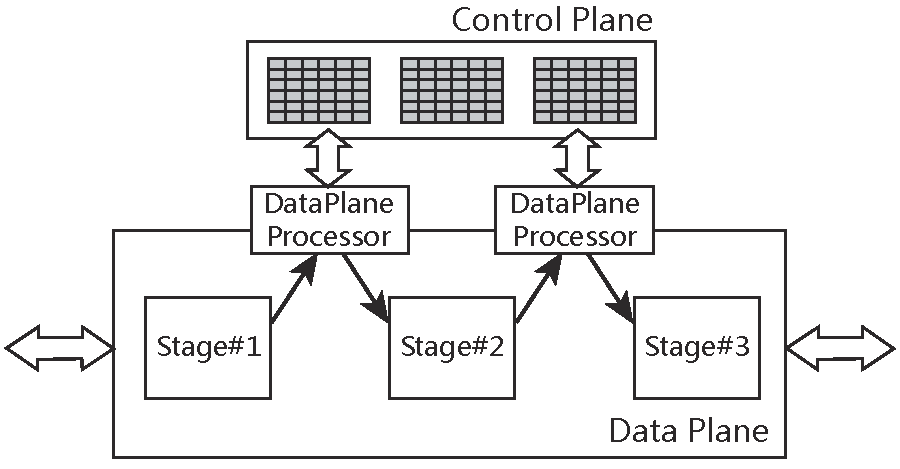
\includegraphics[width=0.6\textwidth]{hwres/pard-dp-arch}
  \caption{可编程数据平面架构}
  \label{fig:pard-dp-arch}
\end{figure}

为解决以上两个问题,本文提出的可编程数据平面架构如图\ref{fig:pard-dp-arch}所示。在PARD中所提出的控制平面/数据平面模型基础上,在数据平面中增加了多个可编程处理器,连接数据平面中其它的逻辑部分,并通过其中的固件代码对数据进行处理。控制平面依然使用三张控制表作为对外访问的接口,通过控制平面网络与集中式的平台资源管理模块通信。由于数据平面部件能够执行代码,因此可以使用软件代码来实现反馈调节,因此触发逻辑已经从控制平面中被移除。
 
要实现以上可编程数据平面架构,需要解决以下三个问题:(1)如何为不同硬件部件的数据平面增加处理器逻辑;(2)处理器如何设计,如何与控制平面进行通信;(3)处理器逻辑如何编程。本文后续章节将针对以上三个问题进行分别阐述。

在讨论数据平面处理器设计前,我们首先以内存控制器和缓存控制器为例,讨论可编程数据平面的设计。

\subsection{内存控制器}
当前的处理器芯片通常会集成2个到4个独立的内存控制器,每个控制器使用独立的内存通道。
每个内存通道连接到多个可并行访问的rank,
而每个rank又是由多个共享地址与数据总线的二维存储阵列(bank)组成。
内存控制器的主要工作就是接收上游的读写请求,并将其转换为下游的DRAM命令,完成数据传输。
以内存控制器作为数据平面,可以在地址映射和访存调度两个位置增加可编程功能。

\textbf{地址映射}\quad
地址映射分为两部分,
首先是通过处理器的页表机制实现了从虚拟地址空间到物理地址空间的映射,
虚拟化场景的出现在这一基础上又增加了扩展页表EPT机制,
额外增加了一级虚拟机物理地址到主机物理地址的映射。
之后是内存控制器将处理器的物理地址空间映射到DRAM阵列中,
通常使用静态地址映射,通过某种固定的规则将物理地址空间映射到DRAM的bank、row和column中。

在PARD架构中,通过在内存控制器前增加MMU模块,通过映射表将不同应用标签的访存请求进行隔离。
但这种方式只实现了一种固定的地址映射机制,即只能进行连续的大块地址分配,
无法实现EPT等技术所支持的细粒度内存空间管理。
为解决这一问题,可以将静态的MMU模块替换为一个处理器,
能够在其中编写软件代码实现地址空间的映射。
通过这种方式除了可以完成PARD中MMU的功能外,还可以实现更细粒度的空间管理,
也可以实现现有虚拟化平台中常见的基于内容的内存空间压缩机制。
除此之外,该处理器还可以通过对请求数据进行额外处理,
以在硬件层面实现更复杂的如数据加密、敏感词过滤等高级功能。

\textbf{访存调度}\quad
在PARD的内存控制平面中,
只实现了简单的基于优先级的访存调度,可以通过增加处理器的方式实现更为灵活的调度策略。
同时也可以像PARDIS\cite{bojnordi_pardis:_2012}工作一样,
将处理器加入到内存控制器内部的请求调度模块中,根据不同应用的需求实现不同的DRAM调度策略。

\subsection{缓存控制器}
Cache控制器的功能是对到达的请求进行缓存操作,使用不同的替换策略,
对数据访问热度进行预测,以提高访存命中率,提高系统性能。
Cache的核心主要包括TagArray、DataArray和替换策略三个部分。
以Cache作为数据平面,可以在容量划分与替换策略两个角度增加可编程功能。

\textbf{容量划分}\quad
传统的Cache并没有提供容量划分功能,
因此不同应用在共享Cache上运行会造成不同程度的干扰。
Intel最新提出的CAT技术\cite{intel-cat}在Cache上增加了按路的缓存容量划分机制。
但按路划分并非适合所有的应用,可以通过使用处理器替换固定的Set/Way映射方式,
根据应用实现更为灵活的缓存容量划分方式。

\textbf{替换策略}\quad
与容量划分的需求类似,不同应用的访存模式不同,
固定的缓存替换策略并不能很好的适应所有应用。因此使用处理器与软件替换策略,
与PARD的应用区分机制结合,可以实现更为灵活高效的缓存。

本章后续章节将依次介绍PARD体系结构中控制平面与数据平面的设计,
并通过模拟器对控制平面的效果进行验证,由于

\section{控制平面设计}

%这里加一个图,说明一下控制平面与硬件的关系,就是大框套小框的关系
控制平面是在硬件之外增加的一层,对硬件的行为进行控制,
同时可以在必要时对发送到硬件的请求进行额外的处理,如地址变换、请求无效等。
由于控制平面能够感知到硬件处理的所有请求,因此可以实现实时性能监控与反馈,
由于控制平面能够对硬件行为进行控制,因此可以实现资源调整机制。

\subsection{实时资源监控与反馈}
资源监控是实现硬件资源可管理共享的第一步,要实现好的共享管理策略,必需对系统当前的资源分配情况、应用性能进行细粒度、实时的监控。
目前监控主要是软件和硬件两个方面,由于


\subsection{资源调整机制}

To facilitate
operators to define resource management policies and program
control planes, PARD provides not only basic priority-based rules
but also an advanced ``trigger$\Rightarrow$action'' programming methodology.

As shown in Figure 3, operators can define several DS-id tag
based “trigger)action” rules each of which targets a set of hardware
resources. Particularly, triggers are based on performance
metrics such as LLC miss rate and are stored in trigger tables; an
action (a.k.a., trigger handler) can be written in any languages as
long as they support file primitives. Operator-defined rules are installed
in the device file tree of the firmware. It is worth noting that
thank to the centralized PRM, trigger and action can be designated
to different resources. For instance, if a trigger is created to monitor
memory bandwidth, its action can be defined to adjust LLC capacity
because LLC miss rate is strongly correlated with both memory
bandwidth and LLC capacity.
Data center operators define actions and “trigger)action” rules
to represent different resource management policies that are correlated
to service-level agreements (SLA) so that users can choose
suitable SLA according to their QoS requirements.


\subsection{控制平面微体系结构设计}


\subsection{控制平面示例}

This subsection presents how to design component-specific control
planes based on the basic control plane structure described in
x3. We focus on the LLC control plane and the memory control
plane, whose microachitecture are shown in Figure \ref{fig:pard-cache-cpdesign}
and Figure \ref{fig:pard-mig-cpdesign}.
If comparing the two figures, we can see that their bottom half
exhibit almost the same structure with only slightly different table
columns. Thus, this basic structure can be easily integrated into a
variety of hardware components,
For I/O devices, we add control planes into I/O bridge and IDE.
Since the design of these I/O control planes is similar to that of the
memory control plane, here we omit their detail design.

\textbf{共享末级缓存控制平面}\quad
图\ref{fig:pard-cache-cpdesign}是共享末级缓存控制平面的微体系结构示意图,
其支持可编程的路划分机制,借助这一机制可以为应用程序调整Cache容量。
该控制平面由三个基本的控制表组成,即参数表、统计表以及触发表,
这三张控制表可以通过可编程接口由PRM上的固件进行访问;
控制平面同时还包括一个连接到PRM的中断线。
除了引入控制平面以外,还需要对原有缓存控制器中的Tag Array以及伪LRU逻辑进行了修改,
所有这些修改均以阴影和虚线的方式在图中进行了标识。

\begin{figure}[tb]
  \centering
  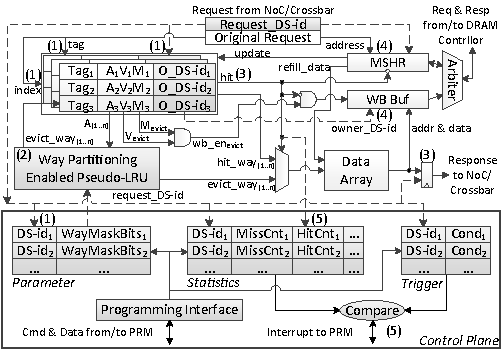
\includegraphics[width=0.7\textwidth]{hwres/pard-cache-cpdesign}
  \caption{共享末级缓存控制平面}
  \label{fig:pard-cache-cpdesign}
\end{figure}

控制平面的引入是否会为共享末级缓存带来额外的延迟是在设计过程中需要考虑的重要问题,
幸运的是目前系统中Cache控制器都是基于流水线设计,
这就使得控制平面的逻辑开销能够隐藏在原有的流水线中,具体流程如下:

(1)当一个包含DS-id和地址的Cache访问请求到达控制器时,
首先需要利用DS-id从参数表中获得相应的路划分掩码。
例如掩码``0x00FF''代表在整个16路中仅使用低端的8路。
与此同时,请求地址被用来在Tag Array中查找相应的条目,
这些条目除了普通的Tag和状态信息以外,还保存有DS-id;

(2)伪LRU逻辑利用参数表输出的掩码以及Tag Array输出的访问历史计算出哪一路需要被替换;

(3)如果请求在缓存中命中,那么数据将从Data Array中取回,
连同请求的DS-id一起通过NoC或者crossbar返回给CPU。
需要注意的是,缓存的命中条件发生了改变,除了请求地址与条目Tag之间原有的约束以外,
还需要请求DS-id与条目DS-id相互匹配。

(4)如果请求在缓存中没有命中,Cache控制器会分配一个MSHR条目,
并在该条目中保存原始请求及其DS-id。
当被请求的数据返回时,Cache控制器需要将MSHR中保存的原始请求DS-id写入到TagArray中。
该DS-id作为``owner DS-id'',在脏数据写回时,
需要与地址和数据一同送入回写缓存,并发送到内存控制器。

(5)在以上各个步骤的过程中,Cache控制平面还会完成以下若干操作:
更新统计表,将Cache使用统计数据发送给平台资源管理器,
在必要时激活触发条件并发出一个中断信号给PRM。
需要特别指出的是这些操作并不在关键路径上,不会对延迟造成影响。

可编程接口用于PRM固件访问该控制平面的三个控制表,
它首先从PRM接收控制表的访问命令,选择相应的表并从指定的表项中读取或写入数据,
更多细节请参见第\ref{chap:prm}章。


\textbf{内存控制器控制平面}\quad
图\ref{fig:pard-mig-cpdesign}是内存控制器控制平面的微体系结构示意图,
为了让PARD的逻辑域抽象能够运行未经修改的操作系统和应用,
该控制平面的参数表保存了用于逻辑域物理地址与DRAM地址的映射信息。
除此之外,控制表中还保存了每个逻辑域的优先级信息用于访存调度。

\begin{figure}[tb]
  \centering
  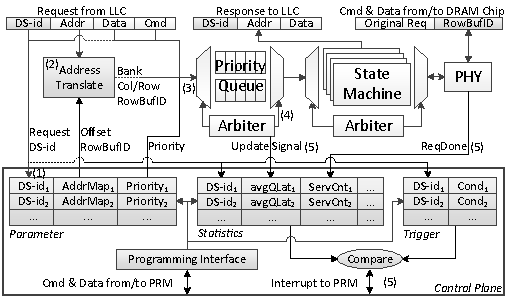
\includegraphics[width=0.7\textwidth]{hwres/pard-mig-cpdesign}
  \caption{内存控制器控制平面}
  \label{fig:pard-mig-cpdesign}
\end{figure}

%Regarding performance isolation, unlike the LLC, the memory
%control plane needs to takes into account two factors, i.e., queuing
%delay and row buffer locality. To manage queuing delay, we add
%a priority queuing mechanism into the memory controller. The
%number of queues depends on the priority levels supported by
%the memory control plane. Our current design only supports two
%priories, but it is easy to extend. To avoid memory low-priority
%requests degrading the row buffer hit rate of high-priority requests,
%we add one extra row buffer into each DRAM chip for high-priority
%memory requests. If we want to augment DRAM chip with more
%buffers, we can leverage some commercial designs such as NEC’s
%virtual-channel memory (VCM).

在性能隔离方面,与Cache控制面不同的是内存控制器控制平面需要考虑以下两个因素:
排队延迟和行缓冲(row buffer)局部性。
为了管理排队延迟,PARD在内存控制器中加入了优先级队列机制,
队列数目取决于内存控制平面能够支持的优先级等级。
当前的设计中暂时仅支持两个优先级,但可以很容易被扩展到多个优先级。
为了防止低优先级访存请求干扰并降低高优先级访存请求的行缓冲命中率,
在DRAM芯片中为高优先级内存请求增加了一个额外的专用行缓冲。
如果需要为DRAM芯片增加更多的优先级控制能力,
可以参考NEC的virtual-channel memory(VCM)技术。

在添加了以上机制后,当一个带有DS-id的内存访问请求到达内存控制器时,
将会顺序引发下列操作:

(1)控制平面利用请求的DS-id从参数表中获得与之相应的地址映射信息、
队列优先级以及行缓冲编号;

(2)请求逻辑域物理地址被转换成DRAM物理地址;

(3)根据控制表中获取的优先级信息将请求连同DS-id置入相应的请求等待队列中;

(4)DRAM调度器根据高优先级优先以及FR-FCFS\cite{rixner_memory_2000}策略从等待队列中选取请求进行服务;

(5)控制平面更新统计表并检查是否满足触发条件,如果满足则发送中断信号到PRM。


\section{可编程数据平面设计}

本节主要讨论可编程数据平面的设计,正如第\ref{}节中所述,
在控制平面的基础上增加数据平面,是为了增强硬件的可编程能力;
同时,PARD的触发机制存在一些问题,主要是

另一方面,PARD中的``trigger$\Rightarrow$action''机制在响应时间上存在瓶颈:
每当触发条件发生后,需要经过控制平面网络将该事件传递到PRM,
由运行在PRM中的软件代码来更新策略,并通过控制平面网络写回到控制平面中。
由于受到控制平面网络延迟以及PRM软件代码延迟的影响,
该机制并不能达到特别高的响应速度。
同时并非所有的触发条件发生后都需要在PRM进行全局处理,
完全可以预定义一些动作,在控制平面本地完成处理。

\subsection{数据平面处理器体系结构}

\begin{figure}[tb]
  \centering
  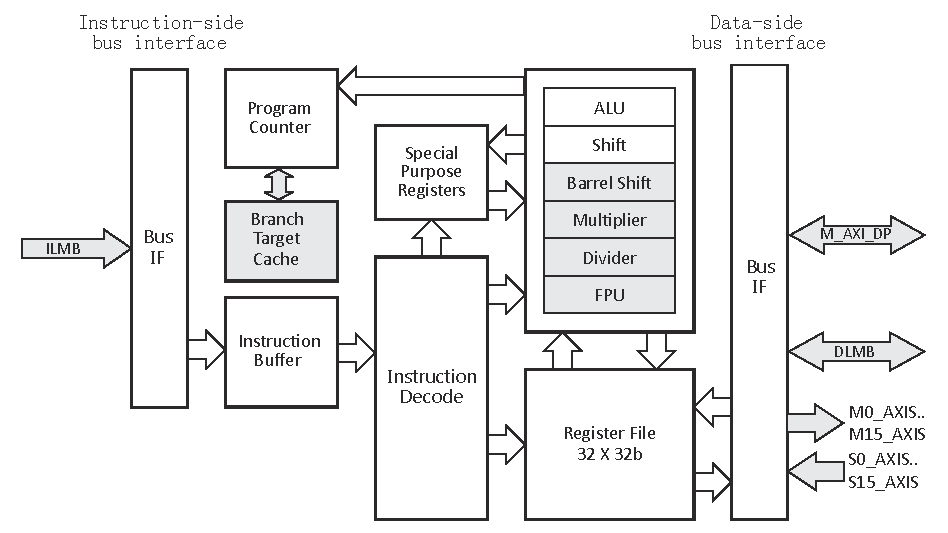
\includegraphics[width=0.8\textwidth]{hwres/pard-dp-proc}
  \caption{数据平面处理器结构图}
  \label{fig:pard-dp-proc}
\end{figure}

由于数据平面处理器位于请求处理的关键路径上,为了保障系统的性能不受影响,需要从以下三个方面进行考虑:
(1)处理器需要执行一系列指令才能完成对请求的处理,因此处理器需要工作在比其所在硬件部件更高频率,以满足硬件部件的性能需求;
(2)处理器的固件代码执行需要确定性,因此不能使用cache结构,而是使用scratchpad memory代替;
(3)由于高频需求,因此处理器功能要尽可能简单,一些必需的复杂的逻辑(如数据压缩与加密等)通过外部加速器的方式进行扩展。

基于以上需求,我们选择使用RISC作为数据平面处理器的基础架构,如图\ref{fig:pard-dp-proc}所示。我们首先对传统RISC架构进行精简,只保留其基本功能,以保证其频率需求;同时增加scratchpad memory作为其指令与数据存储,增加请求缓存接口用于接入硬件设备中,增加控制平面接口用于连接控制平面。
从第2章可知,对于内存控制器与Cache,该处理器的主要工作包括:对请求进行调度、地址变换,对数据进行处理,生成控制信号(如Cache缓存与替换)。要完成以上工作,该处理器需要具备基本的处理器功能外,还需要在数据类型、存储模型和指令上进行扩展。


\subsubsection{数据类型}

数据平面处理器中执行的算法代码大都只是对输入的请求进行处理,因此我们只有``无符号整数''和``请求''两种数据类型,如图\ref{fig:pard-dp-datatype}所示。无符号整数的长度与处理器的位宽相同,都被设置为其所属硬件的位宽,以节约请求处理时位宽转换的开销,保障请求处理的效率。

\begin{figure}[H]
  \centering
  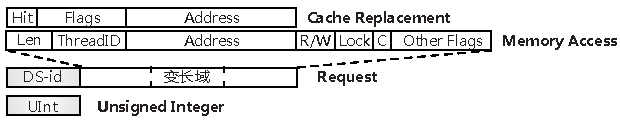
\includegraphics[width=0.7\textwidth]{hwres/pard-dp-datatype}
  \caption{数据平面处理器支持的数据类型}
  \label{fig:pard-dp-datatype}
\end{figure}
 
``请求''类型的是一个变长数据类型,其中包含了固定的16位应用标签(DSid)以及变长的请求数据。以访存请求为例,其中包含请求地址、长度、线程号、读写类型、锁与缓存状态等其它一些标志位;对于Cache替换请求,其中包含了请求地址、Hit/Miss标记以及其它一些标志位等信息。图\ref{fig:pard-dp-datatype}给出了访存请求以及Cache替换请求类型的示例。数据平面处理器本身并不关心请求类型中具体每个位的意义,而只是将其做一个整体进行处理,对每个域的解析或修改由其运行的固件代码完成。

\subsubsection{存储模型}
数据平面处理器中程序员可见的存储结构包含寄存器、请求缓存、scratchpad memory、I/O地址空间四部分。与传统的RISC架构相同,数据平面处理器包含32个通用寄存器(R0-R31),用于进行算数逻辑运算,其中R0是常数零;除此之外,增加了4个用于保存``请求''类型数据的请求寄存器(S0-S3),可以通过请求缓存操作指令(rbget和rbput,参见3.3节),将请求输入队列中的请求读取到该寄存器、或将该寄存器中的请求加入到请求输出队列中;请求寄存器不能直接参与算术逻辑计算,需要先将其部分数据读取到通用寄存器后才能执行计算;请求寄存器之间可以直接进行数据交换。处理器执行的固件代码与数据保存在scratchpad memory中,需要用户自行管理。控制平面被映射为数据平面处理器的外设,提供处理器的固件代码ROM以及处理器的对外接口。

\subsubsection{指令集}
数据平面处理器使用RISC标准的算数逻辑、控制流和访存指令,并在其基础上额外增加了请求缓存操作指令。

请求缓存分为两部分,一个输入缓存一个输出缓存。其中输入缓存既可作为FIFO操作,也可基于DSid进行内容寻址;输出缓存只能作为FIFO操作。用于请求缓存操作的指令如表\ref{tab:pard-dp-isa}所示,指令rbput可以将指定请求寄存器中的请求添加到输出缓存队列末尾;指令rbget有两种使用方式,一种是将输入缓存作为FIFO,取出队列头的请求到请求寄存器,另一种是通过应用标签(DSid)对请求进行筛选,取出第一个满足应用标签的请求到请求寄存器。指令rbcp用于在请求寄存器之间传送数据。指令mfrb用于将请求寄存器中的部分数据传送到通用寄存器;指令mtrb与之相反,用于将通用寄存器的数据传送到请求寄存器指定的位置。

% 数据平面处理器扩展指令
\begin{table}[htb]
  \centering
  \begin{minipage}[t]{0.95\linewidth}
  \caption{数据平面处理器扩展指令}
  \label{tab:pard-dp-isa}
    \begin{tabular*}{\linewidth}{lll}
      \toprule[1.5pt]
      {\heiti 指令} & {\heiti 用途} \\
      \midrule[1pt]

      \multirow{2}{*}{\textbf{rbput}} & \multicolumn{2}{l}{将请求寄存器中的请求增加到请输出请求缓存FIFO队尾。示例:}          \\
                                      & \textit{rbput rb0, s0      } & \textit{\#将s0加入到rb0队尾                          } \\
      \hline
      \multirow{3}{*}{\textbf{rbget}} & \multicolumn{2}{l}{从输入请求缓存读取一个请求到指定的请求寄存器。示例:}              \\
                                      & \textit{rbget s0, rb0      } & \textit{\#从rb0获得第一个请求到s0寄存器              } \\
                                      & \textit{rbget s0, rb0, DSid} & \textit{\#从rb0获得第一个DSid为给定值的请求到s0寄存器} \\
      \hline
      \multirow{2}{*}{\textbf{rbcp}}  & \multicolumn{2}{l}{请求缓存寄存器之间传递数据}                                        \\
                                      & \textit{rbcp s0, s1        } & \textit{\#将s1的值传递给s0                    }        \\
      \hline
      \multirow{3}{*}{\textbf{mfrb,mtrb}}   & \multicolumn{2}{l}{请求缓存寄存器与通用寄存器之间传递值。示例:}                \\
                                      & \textit{mfrb r4, s0, 0     } & \textit{\#将s0第一个32位数据送到r4寄存器      }        \\
                                      & \textit{mtrb s1, r5, 1     } & \textit{\#将r5寄存的数据送到s1寄存器第二个32位}        \\
      \bottomrule[1.5pt]
    \end{tabular*}\\[2pt]
  \end{minipage}
\end{table}

\subsection{固件代码示例}
本节将以三段不同功能的固件代码为例,介绍数据平面处理器的编程方法。

\textbf{段式地址映射}\ 本示例用于实现PARD的内存控制器控制平面所提供的地址映射功能,该功能只需要对访存请求的地址进行修改,而请求的数据无需修改,我们将地址与数据分开由两个处理器进行处理,如图\ref{fig:pard-dp-ex-mapping}右所示。对于数据处理器,其固件代码只使用rbget/rbput指令对请求进行转发。地址处理器首先需要使用rbget指令获取当前请求到请求寄存器,并使用mfrb指令将其中的地址与DSid读取到通用寄存器;而后通过查表的方式获得该请求对应的映射目的地址的基址,对请求地址进行变换,并使用mtrb指令将变换后的地址写回到请求寄存器,最后通过rbput指令将新的访存请求从处理器中送出,完成地址映射功能。

\begin{figure}[H]
  \centering
  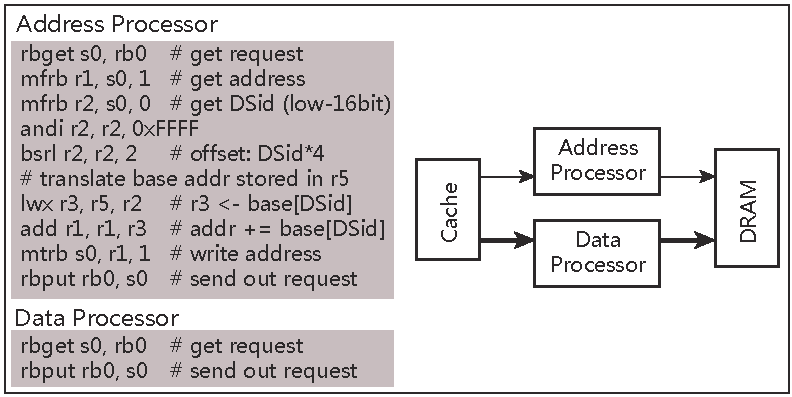
\includegraphics[width=0.7\textwidth]{hwres/pard-dp-ex-mapping}
  \caption{段式地址映射示例}
  \label{fig:pard-dp-ex-mapping}
\end{figure}
 
\textbf{数据加密}\ 本示例实现访存数据加密功能,由于数据加密操作通常需要耗费很长的时间,而且我们的数据平面处理器提供的指令集并不足以完成该操作。因此我们在外部实现了硬件AES加密模块,并通过请求接口将其连接到数据平面处理器上,该结构如图\ref{fig:pard-dp-ex-aes}所示。基于该结构,数据处理器只需要将数据发送到AES模块并等待其完成加密,将加密后的数据送出处理器即可。数据解密与加密过程类似,只需将数据发送到连接有解密模块的请求接口即可。

\begin{figure}[H]
  \centering
  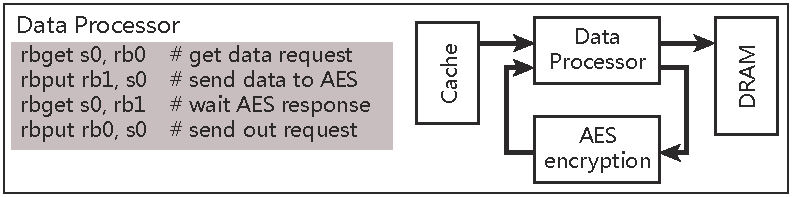
\includegraphics[width=0.7\textwidth]{hwres/pard-dp-ex-aes}
  \caption{访存数据加密示例}
  \label{fig:pard-dp-ex-aes}
\end{figure}
 
\textbf{缓存替换策略}\ 本示例实现缓存替换策略功能,使用可编程处理器替换Cache中原有的LRU模块,使用软件实现基于二叉树的伪LRU替换策略。如图\ref{pard-dp-ex-cache}所示,处理器固件代码工作流程如下:(1)处理器收到Cache前端的请求后,以及Hit/Miss信息,如果缓存命中则无需任何额外操作;(2)对于缓存缺失的请求,首先从地址中解析出tag与set信息,并将解析后的set地址发送到Tag Array,等待其返回该set的信息;(3)根据TagArrary返回的set信息,以及内部的数据结构生成替换目标;(4)将替换目标送出处理器。

\begin{figure}[H]
  \centering
  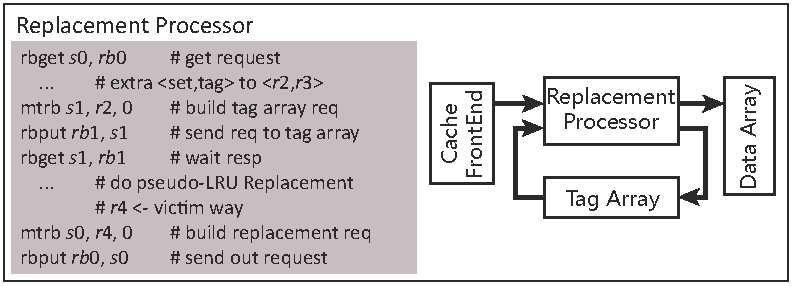
\includegraphics[width=0.7\textwidth]{hwres/pard-dp-ex-cache}
  \caption{缓存替换策略示例}
  \label{fig:pard-dp-ex-cache}
\end{figure}


\section{模拟器验证}

使用模拟器对控制平面以及缓存划分功能进行验证,数据平面由于模拟速度太慢,直接在FPGA平台上进行验证,更多关于FPGA平台的信息参见第\ref{chap:impl}章。


\subsection{模拟器评测结果}

\subsubsection{``Trigger$\Rightarrow$Action'' Mechanism Verification}\leavevmode

We partitioned the server into four LDoms and ran latency-critical memcached
in LDom0. Because the simulation speed is too slow to simulate
network environments, we ran both memcached
client and server in one LDom where they share a CPU core. Although
the client and server may contend for resources within a LDom, this contention
in a blackbox is acceptable while we focus on the interference between LDoms.
The other three LDoms all ran STREAM microbenchmark.

Figure \ref{fig:pardsim:memcached-resptime} illustrates the change of
memcached's tail response time over different request loads.
When memcached runs in the solo-mode (only LDom0 is active),
it can serve 22.5K request per
second (RPS) with reasonable 95-percentile response time (0.6ms). However,
only one CPU core is fully busy, thus the total server CPU utilization is 25\% .
If the other three LDoms are launched to share resources with LDom0,
All four CPU cores are fully busy so that the server exhibits 100\% CPU utilization.
Unfortunately, the throughput of memcached drops to 15K RPS while
the 95-percentile response time already exceeds 1ms. When 
the throughput increases to 20K RPS, the 95-percetile response time
dramatically increases by two orders of magnitude (62.6ms). 

To verify the the effectiveness of the ``\emph{trigger$\Rightarrow$action}'' mechanism,
As shown in Figure \ref{fig:programming}, we predefined a trigger for LDom0, i.e.,
``LLC.MissRate $>$ 30\% $\Rightarrow$ increasing LLC capacity up to 50\%''.

Next we installed the LLC trigger into the LLC control plane before launching
LDom0 and then launched all four LDoms. Figure \ref{fig:pardsim:memcached-20krps-missrate} shows how
LDom0's LLC miss rate varies while the trigger takes effect. After half of LLC capacity is
dedicated to LDom0, memcached's LLC miss rate quickly decreases to
only about 10\%, just slightly larger than the solo-mode's miss rate (7\%).
As a result, the throughput increases to 22.5K RPS with reasonable
95-percentile response time (1.2ms). Compared with the solo-mode, 
since LDom0 uses only half of LLC capacity, this tail response time is 
slightly longer. Overall, these experimental results show that even the total 
server CPU utilization is 100\% (all four cores are fully busy),
memcached's behaviors can still approach the solo mode.

This experiment demonstrates that the ``\emph{trigger$\Rightarrow$action}'' mechanism 
is able to take the advantage of PARD and is beneficial for balancing the trade-offs between
resource utilization and applications' QoS.


\subsubsection{Disk I/O Performance Isolation}\leavevmode

PARD is able to manage not only capacity resources (e.g., LLC)
but also bandwidth resources such as memory and I/O bandwidth.
In this experiment, two LDoms are active and each LDom executes
disk write operation through
this command: ``\emph{dd if=/dev/zero of=/dev/sdb bs=32M count=16}''.

Initially, two LDoms share the IDE controller so that they exhibit the same
disk I/O bandwidth. Assume the user of LDom1 pays more money in order to get
better I/O performance, we manually ran
``\emph{echo 80 $>$ /sys/cpa/cpa3/ldom0/parameters/bandwidth}''
to program the IDE control plane
to increase the disk I/O bandwidth quota of LDom0 to 80\%.
Figure \ref{fig:pardsim:iosched} illustrates the effect of disk I/O
bandwidth reallocation.

Although there are other approaches to manage I/O bandwidth such as cgroup \cite{cgroup},
PARD provides a more efficient fine-grained I/O management scheme that requires
no modifications to OS kernel and applications, reducing the complexity of software
stack.

\begin{figure}[tb]
\begin{minipage}{0.48\textwidth}
  \centering
  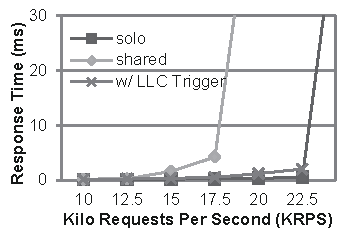
\includegraphics[height=4.5cm]{hwres/pard-sim-memcached-resptime}
  \caption{模拟器memcached 95\%-tail延迟示意图}
  \label{fig:pardsim:memcached-resptime}
\end{minipage}\hfill
\begin{minipage}{0.48\textwidth}
  \centering
  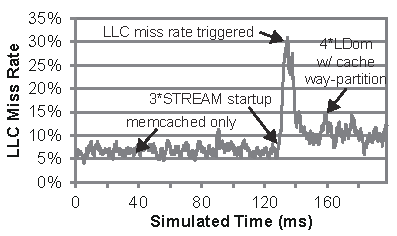
\includegraphics[height=4.5cm]{hwres/pard-sim-memcached-20krps-missrate}
  \caption{模拟器memcached末级缓存命中率变化(20KRPS)}
  \label{fig:pardsim:memcached-20krps-missrate}
\end{minipage}
\end{figure}

\begin{figure}[tb]
  \centering
  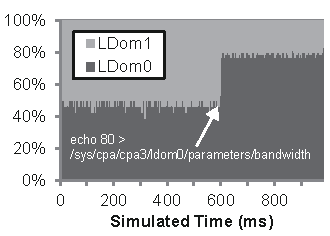
\includegraphics[width=0.5\textwidth]{hwres/pard-sim-iosched}
  \caption{磁盘I/O性能隔离}
  \label{fig:pardsim:iosched}
\end{figure}

\section{小结}

